\documentclass[11pt, a4paper]{article}

%%% SST LAB PROTOCOLL PREAMBLE
%%% 2019
%%%%%%%%%%%%%%%%%%%%%%%%%%%%%%%


%%% PACKAGES
%%%%%%%%%%%%%%%%%%%%%%%%%%%

\usepackage[ngerman]{babel}

\usepackage[utf8]{inputenc}
\usepackage{amsmath}
\usepackage{pgfplots}
\usepackage{tikz}
\usepackage[many]{tcolorbox}
\usepackage{graphicx}
\graphicspath{ {./graphics/} }
\usepackage{pdfpages}
\usepackage{dashrule}
\usepackage{float}
\usepackage{siunitx}
\usepackage{trfsigns}
\usepackage{booktabs}
\usepackage[european]{circuitikz}
\usepackage{tcolorbox}

%%% DOCUMENT GEOMETRY
%%%%%%%%%%%%%%%%%%%%%%%%%%%

\usepackage{geometry}
\geometry{
 a4paper,
 total={0.6180339887498948\paperwidth,0.6180339887498948\paperheight},
 top = 0.1458980337503154\paperheight,
 bottom = 0.1458980337503154\paperheight
 }
\setlength{\jot}{0.013155617496424828\paperheight}
\linespread{1.1458980337503154}

\setlength{\parskip}{0.013155617496424828\paperheight} % paragraph spacing


%%% COLORS
%%%%%%%%%%%%%%%%%%%%%%%%%%%

\definecolor{red1}{HTML}{f38181}
\definecolor{yellow1}{HTML}{fce38a}
\definecolor{green1}{HTML}{95e1d3}
\definecolor{blue1}{HTML}{66bfbf}
\definecolor{hsblue}{HTML}{00b1db}
\definecolor{hsgrey}{HTML}{afafaf}

%%% CONSTANTS
%%%%%%%%%%%%%%%%%%%%%%%%%%%
\newlength{\smallvert}
\setlength{\smallvert}{0.0131556\paperheight}


%%% COMMANDS
%%%%%%%%%%%%%%%%%%%%%%%%%%%

% differential d
\newcommand*\dif{\mathop{}\!\mathrm{d}}

% horizontal line
\newcommand{\holine}[1]{
  	\begin{center}
	  	\noindent{\color{hsgrey}\hdashrule[0ex]{#1}{1pt}{3mm}}\\%[0.0131556\paperheight]
  	\end{center}
}

% mini section
\newcommand{\minisec}[1]{ \noindent\underline{\textit {#1} } \\}

% quick function plot
\newcommand{\plotfun}[3]{
  \vspace{0.021286\paperheight}
  \begin{center}
    \begin{tikzpicture}
      \begin{axis}[
        axis x line=center,
        axis y line=center,
        ]
        \addplot[draw=red1][domain=#2:#3]{#1};
      \end{axis}
    \end{tikzpicture}
  \end{center}
}

% box for notes
\newcommand{\notebox}[1]{

\tcbset{colback=white,colframe=green1!100!black,title=Note!,width=0.618\paperwidth,arc=0pt}

 \begin{center}
  \begin{tcolorbox}[]
   #1 
  \end{tcolorbox}
 
 \end{center} 
 
}

% box for equation
\newcommand{\eqbox}[2]{
	
	\tcbset{colback=white,colframe=green1!100!black,title=,width=#2,arc=0pt}
	
	\begin{center}
		\begin{tcolorbox}[ams align*]
				#1
		\end{tcolorbox}
		
	\end{center} 
	
}
% END OF PREAMBLE

\newcommand{\code}[1]{{\lstinline{#1}}}



%-------------------------------------------------------------------------------
\begin{document}

\begin{center}
  \Large{Host-to-Host-Kommunikation im Rahmen der Netzwerkprogrammierung}
\end{center}

\begin{flushright}
  R. Grünert\\
  S. Klobe\\
  \today
\end{flushright}

Zur erfolgreichen Kommunikation zwischen zwei Hosts mit z. B. \code{echotcp}
bzw. \code{daytimetcp} über das Internet bedarf es mehrerer
Konfigurationsschritte. Die notwendigen Schritte werden in diesem Dokument
erklärt. Hier eine Zusammenfassung:

\begin{itemize}

  \item Vor Beginn der Einstellungen sollte ein fester Port für den Serversocket
        im jeweiligen Serverprogramm angelegt werden. In unserem Fall ist dies
        der Port \code{44203}.

  \item Damit der Server über das Internet erreichbar ist (also vom
        Client-Programm innerhalb eines anderen Netzwerkes), wird eine
        öffentliche IPv4-Adresse benötigt.

  \item Am Gateway des Servernetzwerkes muss mittels Portweiterleitung der
        eingehende Traffic des Clients auf z.B. Port \code{44203} an den
        Server-Host weitergeleitet werden.

  \item Die Firewall des Server-Hosts muss für den Serverport geöffnet sein.

  \item Bei Verwendung einer virtuellen Maschine muss dort ebenfalls der Port
        weitergeleitet werden.

\end{itemize}

Zusätzlich kann das freie Programm \textit{Wireshark} dabei helfen,
Kommunikationsprobleme zu identifizieren.\\

Abb. \ref{beep} zeigt eine vereinfachte Darstellung der Situation.

\begin{figure}[H]
\centering
\resizebox{0.618\textwidth}{!}{\import{graphics/}{topo.pdf_tex}}
\caption{Stark vereinfachte Darstellung der Netztopologie}\label{beep}
\end{figure}

%-------------------------------------------------------------------------------
\section{IPv4 Adresszuweisung}

Da im Modul ENP die Netzwerkkommunikation auf Schicht 3 über IPv4 gelehrt wird,
benötigt zumindest der Server-Host eine solche öffentliche Adresse.
Da man heutzutage bei den meisten Providern mit \emph{Dual Stack Lite}
angebunden wird und daher nur eine IPv6-Adresse erhält, ist in diesem Fall eine
Anfrage beim Provider nötig, um eine IPv4 Adresse zugewiesen zu bekommen.
Im Falle unseres Providers (Vodafone) erfolgte dies durch einen einfachen Anruf.\\

Gelingt keine IPv4-Zuweisung, bleiben nur Ausweichmöglichkeiten, wie z.B. die
VPN-Verbindung beider Netzwerke.\\

Mithilfe einer Website zur Ermittlung der eigenen öffentlichen IP-Adresse kann
im vorher-nachher-Vergleich die Zuweisung überprüft werden
\footnote{z. B. mit https://www.whatismyip.com/}.

%-------------------------------------------------------------------------------
\section{Port-Forwarding}
Aus Sicht des inside-global Netzwerkes gibt es noch keine Möglichkeit,
um den Server von anderen Hosts im Heimnetzwerk zu unterscheiden.
Der Router sollte daher so konfiguriert werden, dass er den Traffic,
der an den Port des Servers gerichtet ist auch an den Server
weiterleitet (Port-Forwarding).

%-------------------------------------------------------------------------------
\subsection{Ermittlung der Router-IP-Adresse}
Über das Webinterface des Routers kann man das Port-Forwarding einstellen. Um
die lokale IP-Adresse des Routers zum Erreichen des Webinterfaces herauszufinden,
gibt es betriebssystemabhängig verschiedene Möglichkeiten.

\paragraph{Router-IP unter Windows}
Über den CMD-Befehl \code{ipconfig} findet man unter dem Eintrag
\glqq Default Gateway\grqq bzw \glqq Standardgateway\grqq die gewünschte
Routeradresse (Abb. \ref{gwin}).

\paragraph{Router-IP unter Linux}
Unter Linux kann man den Befehl \code{ip r} oder \code{ip route} nutzen, um die
Routeradresse herauszufinden.

%-------------------------------------------------------------------------------
\subsection{Aufruf des Webinterfaces}
Über die oben ermittelte IP-Adresse kann man im Browser das Webinterface des
Routers aufrufen. Das Passwort findet man i.d.R. auf dem Router selbst.

%-------------------------------------------------------------------------------
\subsection{Einstellung des Port-Forwardings}
Die genaue Einstellung des Port-Forwardings unterscheidet sich natürlich je nach
Gerät, im allgemeinen müssen dann aber nur ein Port(bereich) und eine gewünschte
Ziel-IP-Adresse angegeben werden. Ein Beispiel ist in Abb. \ref{forv} zu sehen.\\

Die Ziel-IP-Adresse ist die lokale Adresse des Hosts auf dem das Serverprogramm
läuft. Man findet sie unter Windows ebenfalls über den \code{ipconfig}-Befehl
und unter Linux z.B. über \code{ip a}. Da die Adresszuweisung meist standardmäßig
über DHCP stattfindet, sollte darauf geachtet werden, dass sich die beim
Port-Forwarding angegebene Adresse ändern und daher eine Neukonfiguration
notwendig sein kann.

\begin{figure}[H]
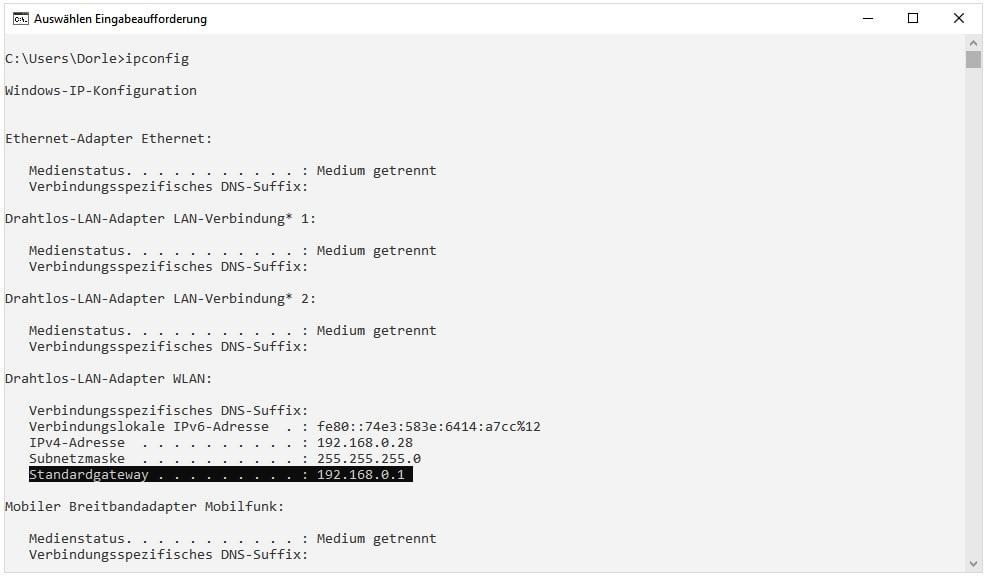
\includegraphics[width=\textwidth]{graphics/gatewayip_windows}
\caption{CMD-Ausgabe des ipconfig-Befehls unter Windows}\label{gwin}
\end{figure}

\begin{figure}[H]
\centering
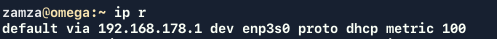
\includegraphics[width=0.618\textwidth]{graphics/gatewayip_linux}
\caption{Ausgabe des ipconfig-Befehls unter Linux}\label{glin}
\end{figure}

\begin{figure}[H]
\centering
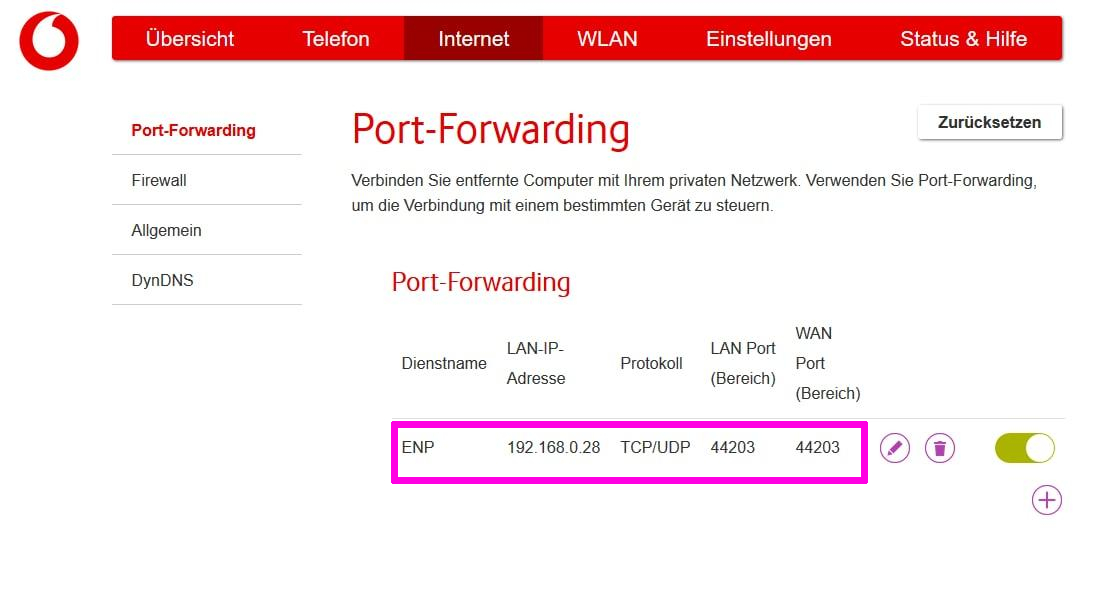
\includegraphics[width=\textwidth]{graphics/forv}
\caption{Beispiel für Port-Forwarding Ansicht eines Vodafone-Routers}\label{forv}
\end{figure}

\section{Firewall}
Dem Paket steht nun noch die Firewall des Serverhosts im Weg. Diese blockiert
i.d.R. den einkommenden Traffic, der an den Port des Serverprogramms gerichtet
ist. Je nach Betriebssystem geschieht das Öffnen des Ports unterschiedlich.
Hier wird sich allerdings auf Windows beschränkt, da dies der Regelfall für
ENP-Teilnehmer*innen ist. Ein Tutorial für das Öffnen von Ports unter Ubuntu
findet man z.B.
\href{https://www.cyberciti.biz/faq/how-to-open-firewall-port-on-ubuntu-linux-12-04-14-04-lts/}{hier}.\\

\subsection{Portregeln unter Windows}
Über \code{Systemsteuerung} $\rightarrow$ \code{System und Sicherheit}
$\rightarrow$ \code{Windows Defender Firewall} $\rightarrow$ \code{Erweiterte
  Einstellungen} gelangt man zu den Portregeln. Mit einem Rechtsklick auf
\code{Eingehende Regeln} und danach auf \code{Neue Regel} kann man den Port des
Servers freigeben. Abb. \ref{fwconfig1} bis \ref{fwconfig2} zeigen eine
Beispielkonfiguration für den Serverport
\code{44203}.

\begin{figure}[H]
\centering
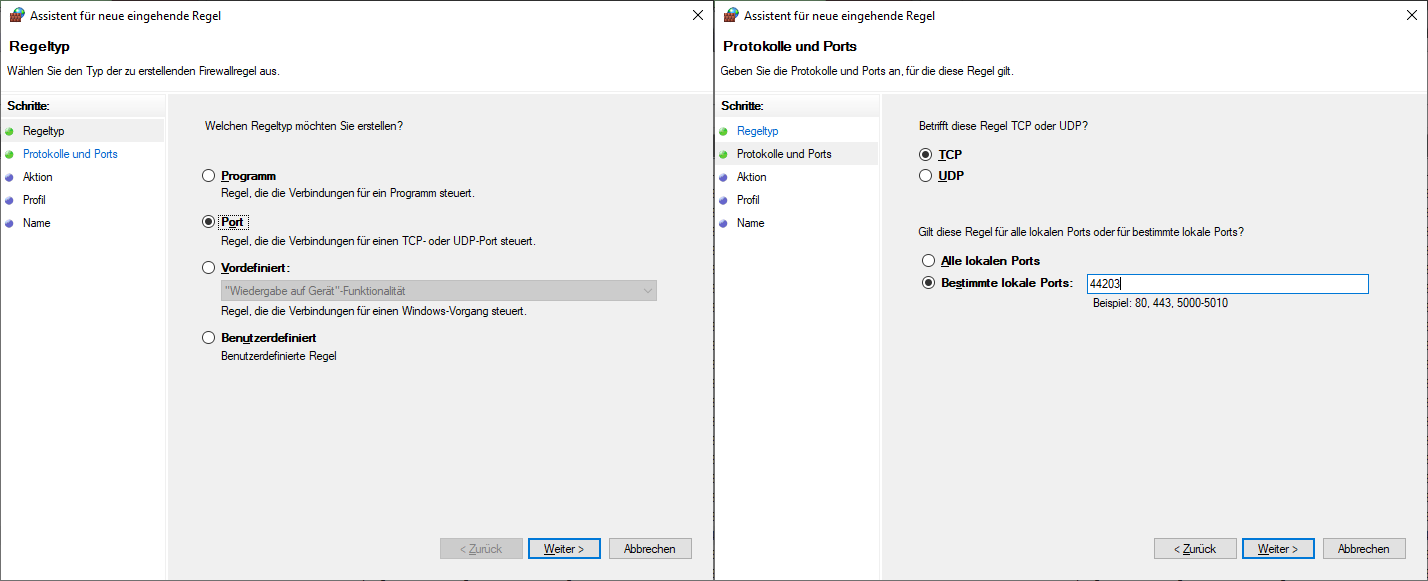
\includegraphics[width=\textwidth]{graphics/fwconfig1}
\caption{}\label{fwconfig1}
\end{figure}

\begin{figure}[H]
\centering
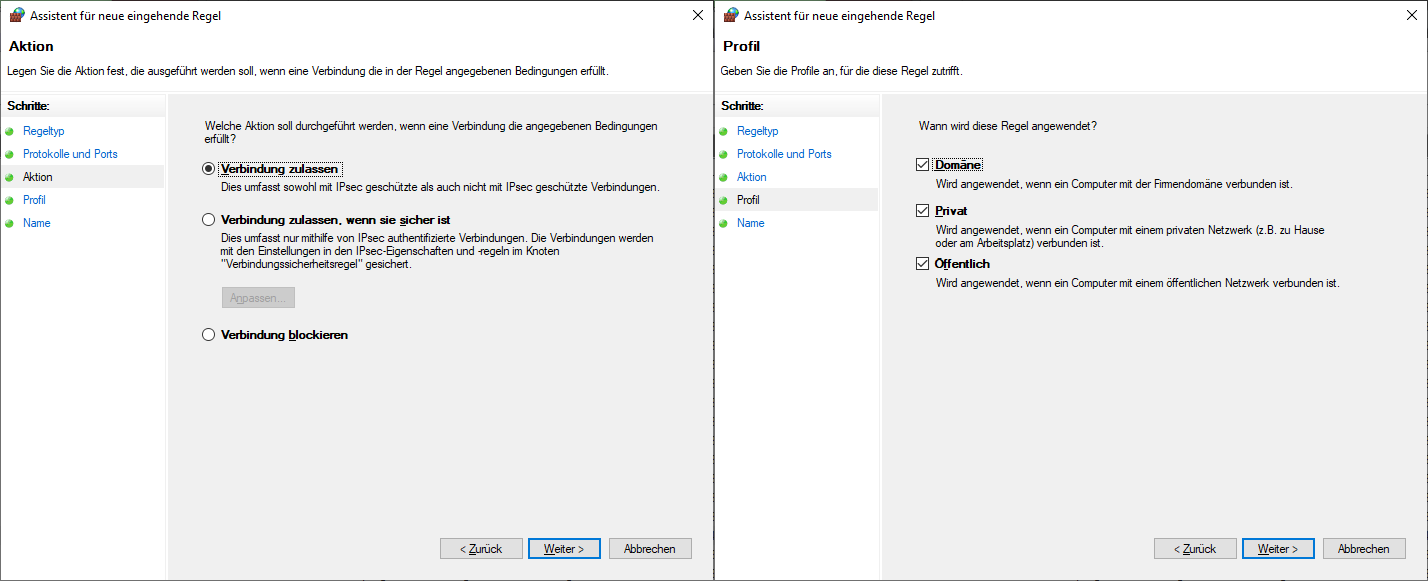
\includegraphics[width=\textwidth]{graphics/fwconfig2}
\caption{}\label{fwconfig2}
\end{figure}

\section{Virtualbox}
Da Teilnehmer*innen des Moduls ENP meist eine virtuelle Maschine
(Oracle VirtualBox) auf Windows nutzen, um unter Linux zu arbeiten, benötigt man
in diesem Fall zusätzliche Konfigurationen unter VirtualBox.\\

Als erstes sollte sichergestellt sein, dass VirtualBox von der Windows-Firewall
ins Netzwerk gelassen wird. Dies kann ebenfalls über
\code{Systemsteuerung} $\rightarrow$ \code{System und Sicherheit}
$\rightarrow$ \code{Windows Defender Firewall} geprüft werden. Alternativ
kann man auch in der virtuellen Maschine testen, ob man z.B. mit einem Browser
eine Website aufrufen kann.\\

Weiterhin muss auch hier eine Portweiterleitung eingerichtet werden.

\subsection{Port-Forwarding}

Die Weiterleitungseinstellungen erreicht man über den \code{Netzwerk}-Tab unter
den Einstellungen der Virtuellen Maschine. Eine Beispielkonfiguration ist in
Abb. \ref{vm_port_fw} zu sehen.

\begin{figure}[H]
\centering
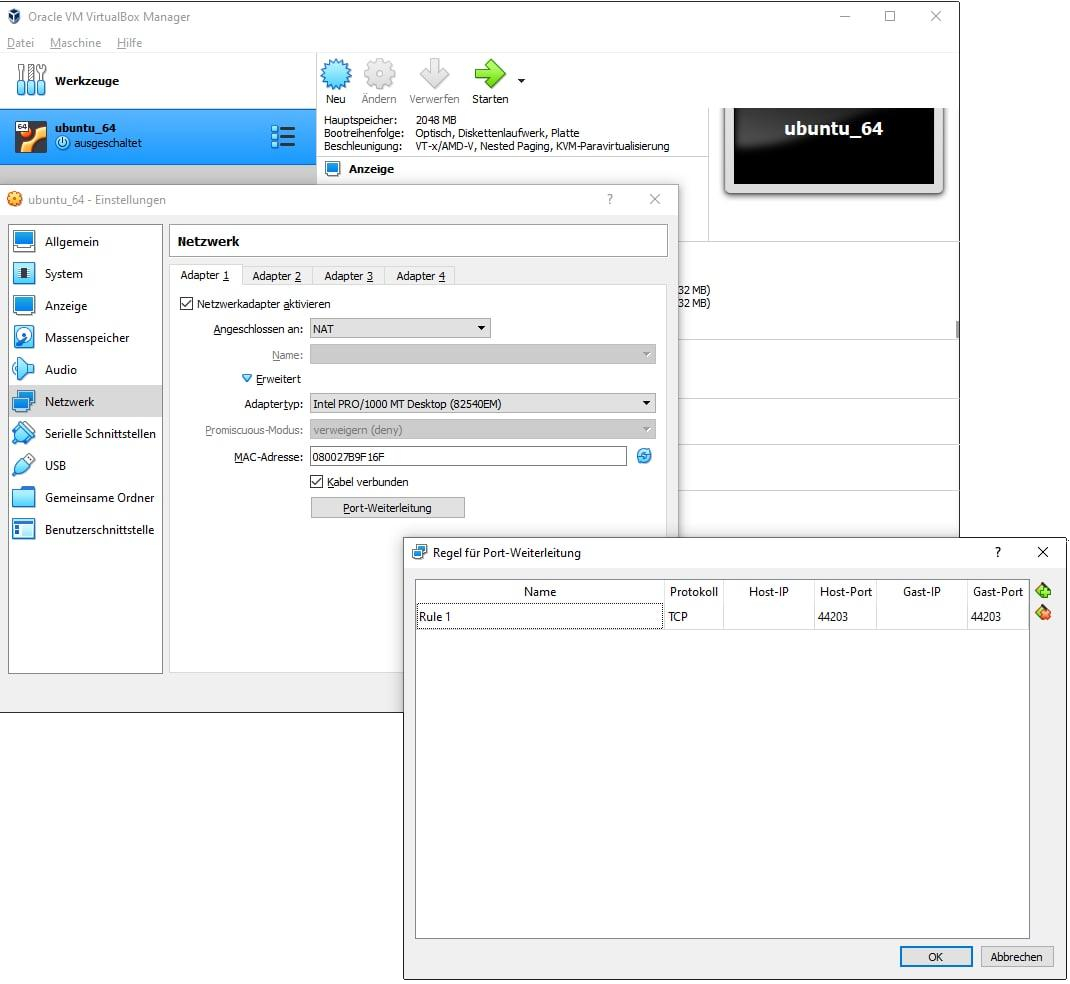
\includegraphics[width=\textwidth]{graphics/vm_port_fw}
\caption{Einstellung der Portweiterleitung unter VirtualBox}\label{vm_port_fw}
\end{figure}

\textbf{Hinweis}: Möglicherweise bedarf es einem Neustart von Windows oder
VirtualBox.

\section{Test}
Nach den oben beschriebenen Schritten kann der erste Test gestartet werden.
Es wird angenommen, dass das Clientprogramm (cli) so geschrieben ist, dass man
über die Aufrufargumente IP-Adresse und Port des Servers angeben kann. Der
Aufruf für unser Beispiel funktioniert dann z.B. so: \code{cli 172.217.14.195
  44203}.\\

An Client- und Serverprogramm sollten keine weiteren Modifikationen
notwendig sein. Der Listen-Socket des Servers sollte am einfachsten mit der
Adresse des Macros \code{INADDR_ANY} gebunden werden.

\section{Troubleshooting}
Mithilfe des Programmes \textit{Wireshark} kann der Netzwerkverkehr
der Netzwerkschnittstellen sowohl beim Client als auch beim Server in Echtzeit
überwacht werden. Mit dem Filterbefehl \code{tcp.port == 44203} können nur die
relevanten Pakete angezeigt werden. Bei Verbindungsaufbau sowie Datenübertragung
(z.B. Senden der Zeichenkette bei \code{echotcp}) erscheinen dann dort die
zugehörigen Pakete.\\

Abb. \ref{fwdoof} sowie Abb. \ref{fwdoof2} zeigen Wireshark-Traces aus
Client- und Serversicht, bei denen die Firewall des Server-Hosts den Client-
Traffic nicht hindurchlässt. Der Client schickt dann kontinuierliche Anfragen
zum Verbindungsaufbau (SYN).\\

Ist das Port-Forwarding am Router nicht korrekt konfiguriert, zeigt der Trace
des Server-Hosts (Abb. \ref{fwdoof2}) keine Pakete an.

\begin{figure}[H]
\centering
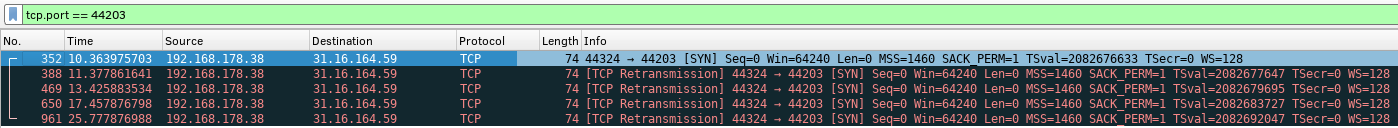
\includegraphics[width=\textwidth]{graphics/firewall_doof}
\caption{Wireshark Trace am Clientrechner bei Firewall-Problemen}\label{fwdoof}
\end{figure}

\begin{figure}[H]
\centering
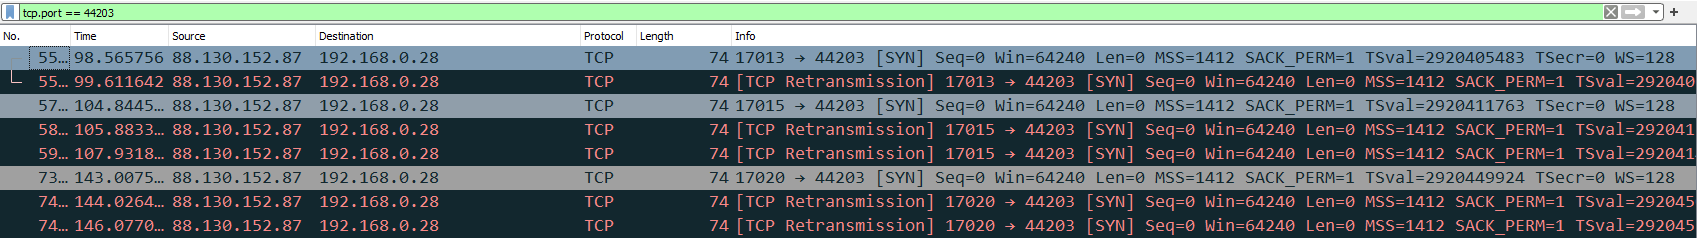
\includegraphics[width=\textwidth]{graphics/firewall_doof_srv}
\caption{Wireshark Trace am Serverrechner bei Firewall-Problemen}\label{fwdoof2}
\end{figure}

Für den Fall, dass die Portfreigabe-Einstellungen unter Windows keine Wirkung haben,
kann auch die gesamte Firewall deaktiviert werden (Abb. \ref{fwaus}).

\begin{figure}[H]
\centering
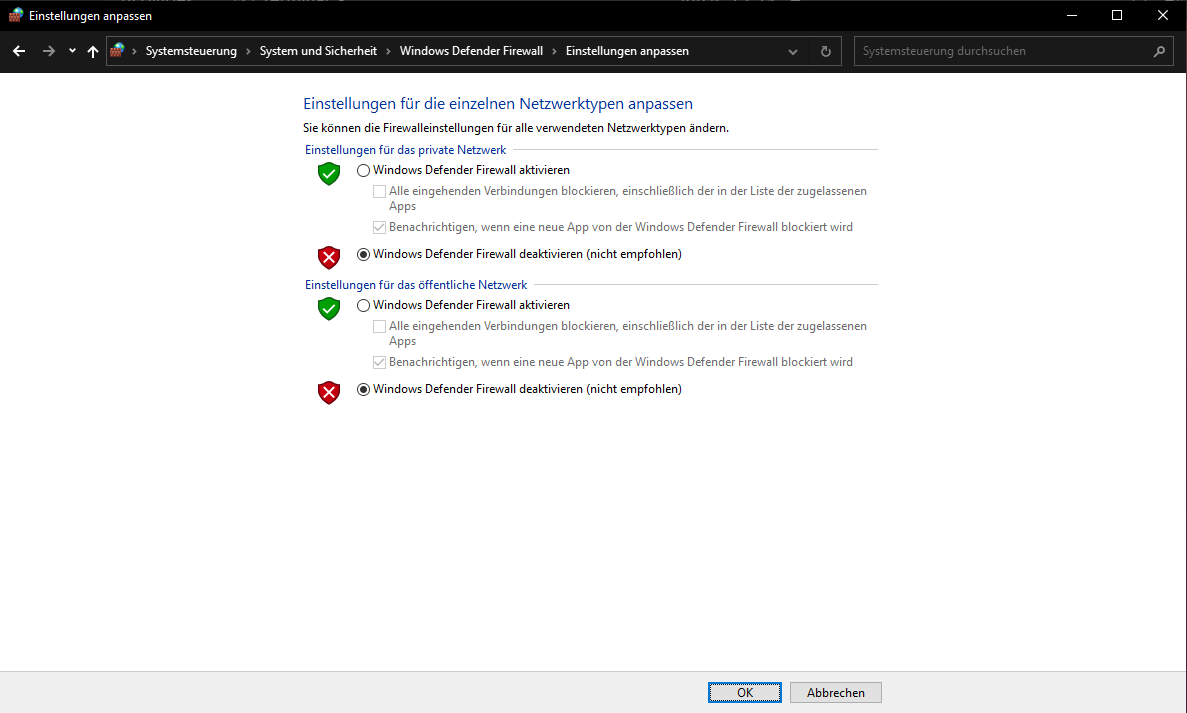
\includegraphics[width=\textwidth]{graphics/firewall_aus}
\caption{}\label{fwaus}
\end{figure}

\section{Verbesserungen / Hinweise}
Unsere Testumgebung bestand aus einem Host mit nativem Linux (Client) und einem
Host mit Linux unter VM auf Windows (Server). Die anderen Kombinationen, sprich
Linux-Client/Windows-Server, Linux-Client/Linux-Server, sowie Windows-Client/
Windows-Server, wurden daher noch nicht getestet. Möglicherweise sind unter diesen
Bedingungen weitere Einstellungen notwendig (z.B. an der Firewall auf dem
Clientrechner).

\end{document}
